\setcounter{equation}{0}
\setcounter{figure}{0}

\section{Calorimetry}

Name \rule{2.0in}{0.1pt}\hfill{}Section \rule{1.0in}{0.1pt}\hfill{}Date
\rule{1.0in}{0.1pt}

\textbf{Objective}

\begin{itemize}

\item To learn to use a method for measuring heat called calorimetry.

\item Measure the specific heat of aluminum and the heat of fusion of ice.

\end{itemize}

\textbf{Apparatus}

\begin{center}
\begin{tabular}{|l|l|l|} \hline
Hypsometer and stand & Hot plate            & Ice \\ \hline
Data Studio software & Temperature probe    & Clamp and stand \\ \hline
Safety goggles       & Aluminum pellets     & Compact scale           \\ \hline
Calorimeter          & Stirrers             &            \\ \hline
\end{tabular}
\end{center}

\textbf{Introduction to Calorimetry} 

Calorimetry is a method for measuring heat. As applied in this experiment,
the method involves the mixing together of substances initially at
two different temperatures. The substances at the higher temperature
lose heat and the substances at the lower temperature gain heat until
thermal equilibrium is reached.

\textbf{Activity \stepcounter{activity}\arabic{activity}: Statement of Conservation of Energy}

If no heat is transferred to the surroundings, what is the relationship
between the heat lost by the substances initially at high temperature
and the heat gained by the substances initially at low temperature?
Note: This is simply a statement of conservation of energy.

\vspace{0.3cm}
{\centering \resizebox*{!}{3.5in}{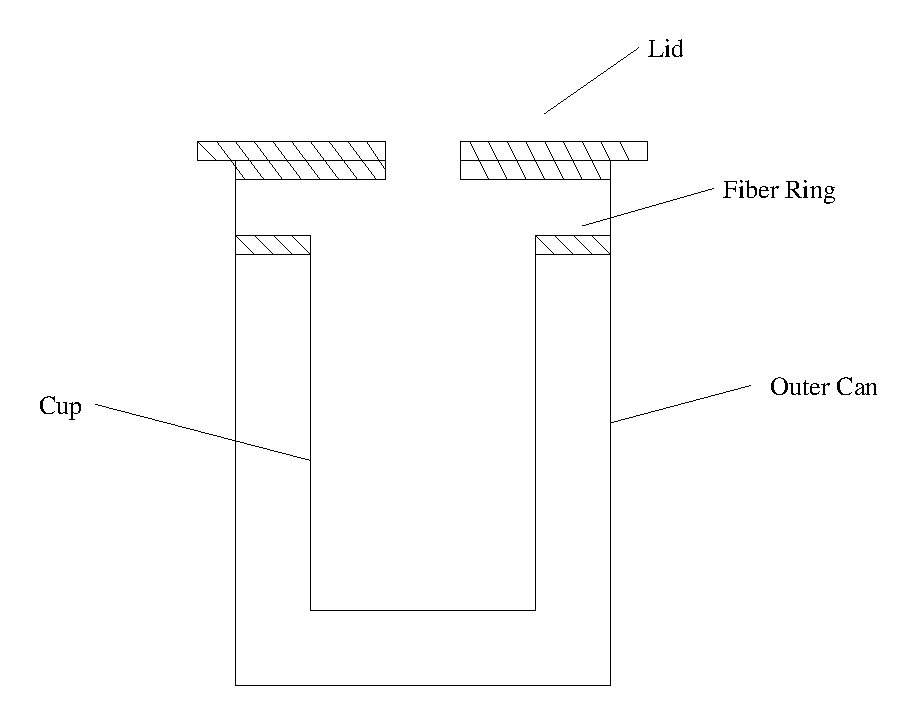
\includegraphics{heat/calorimetry_fig_1.eps}}  \par}
\vspace{0.3cm}

\textbf{Experimental Equipment} 

A calorimeter, shown in the above figure, is used in this experiment
to minimize the exchange of heat between the system and the surroundings.
The inner calorimeter cup is thermally insulated from the surroundings
by suspending it on a ring of material with low heat conductivity
and surrounding it with a layer of air. Also the cup is shiny to minimize
radiation loss. Hence, if the mixture of substances is placed inside
the calorimeter cup, the heat lost to or gained from the surroundings
can be ignored, and the above relationship can be used. The only part
of the calorimeter which is involved in the calculation is the inner
calorimeter cup which contains water and in which an exchange of heat
between the hot and cold bodies takes place. The cup will undergo
the same temperature change as the contained water. Of course, an
instrument will have to be introduced to measure the temperature of
the system, but the heat gained or lost by the instrument is small
and can be ignored.

\textbf{Activity \stepcounter{activity}\arabic{activity}: Specific Heat of Aluminum}

(a) Fill the hypsometer (boiler) at least half full of water and start
heating the water.

(b) Determine and record the mass of the hypsometer cup, m\( _{h} \).
Then fill it about half full with dry aluminum pellets. Determine
and record the mass of the cup and pellets, m\( _{hp} \), and calculate
the mass of the pellets, m\( _{p} \). Record the measurements in
the space below.
\vspace{15mm}

(c) Fill the plastic beaker with ice water. Open the \textit{Calorimetry}
application in the 132 Workshop folder in the {\bf Start} menu and start
collecting data. To make sure the temperature probe is working 
properly place it in the ice water and
check that it is reading approximately 0\( ^{\circ } \)C. If not,
then consult your instructor.

(d) Place the hypsometer cup in the top of the hypsometer and put the 
temperature probe into the middle of the pellets.  
To do this, remove the pellets from the cup, place the temperature probe in 
the proper position (using the clamp and stand), then return the pellets to the cup.

(e) Determine and record the mass of the calorimeter cup, m\( _{c} \).
Fill this cup about half full of cold tap water. Determine and record
the mass of the cup and water, m\( _{cw} \), and calculate the mass
of the water, m\( _{w} \). Then place the calorimeter cup in the outer
can and put the lid on.
\vspace{15mm}

(f) When the temperature of the pellets becomes constant, at or near
100\( ^{\circ } \)C, record the temperature of the pellets as T\( _{p} \).
Remove the probe from the pellets and put it in the cold water in the calorimeter cup. 
When the temperature of the water levels off, record it as T\( _{w} \).
\vspace{15mm}

(g) Now, quickly but carefully, pour the pellets into the water in
the calorimeter cup. Stir the water occasionally with the temperature probe and
monitor the temperature of the mixture. When the temperature levels off, record
this value as T. Click the {\bf Stop} button on the monitor, 
print your graph of temperature as a function of time and include it in this unit.
\vspace{15mm}

\newpage 

(h) Write the complete heat equation and solve for the unknown specific
heat of the metal. 
The specific heat of the calorimeter cup is 900 J/kg-\( ^{\circ } \)C.
\vspace{2in}

(i) Collect the other measurements of the specific heat from the other groups in
the class. 
Look up the accepted value for the specific heat of aluminum and
calculate the difference  between this value and the average.
Do the two values agree within experimental uncertainties?
Comment on possible sources of error.
\vspace{20mm}

